\section{Evaluation}
\label{sec:flakycat-evaluation}

In this section, we explain our evaluation setting for FlakyCat.
First, we describe our data curation process, then, we present our approach for answering each of the three research questions. 

\subsection{Data Curation}
\label{dataset}

\subsubsection{Collection}
For our study, we had to collect a set of flaky tests containing their source code and their flakiness category.
We focused our collection efforts on one programming language, as training a classifier using code and tokens from different programming languages is more challenging. 
For the language choice, we opted for Java, which is the most common language in previous flakiness studies (and thus datasets). 
To increase the amount of data used in this study, we also collected a new set of flaky tests mined from GitHub that we classified manually.

\paragraph{Existing datasets} 

\begin{table}[htbp]
\centering
\caption{Data filtering performed on the different datasets used in this study. Collected represents the new dataset we retrieved.}
\begin{tabular}{c|c|c|c|c|c}
\toprule 
\multirow{2}{*}{\textbf{Filters}} & \multicolumn{5}{c}{\textbf{Datasets}} \\
\cmidrule{2-6} 
&  \cite{Luo2014} & \cite{across_pr} & \cite{habchiPinpointing} & \cite{Shi2019iFix} & Collected \\ 
\midrule 
\textbf{Inspected commits} & 201 & 170 & 40 & 101 & 270\\ 
 Commit not found  & 12 & 12 & 4 & 3 & 3\\
 Duplicated commit & 0 & 2 & 0 & 0 & 3 \\ 
 Open commit & 0 & 0 & 0 & 33 & 0 \\
Flaky test not found & 45 & 21 & 13 & 0 & 42 \\ 
Configuration problems & 3 & 8 & 0 & 0 & 0\\
Not Java & 15 & 5 & 0 & 0 & 8 \\ 
Category hard to classify & 40 & 57 & 4 & 0 & 22 \\ 
\textbf{Considered commits} & 86 & 65 & 19 &  65 & 192\\
\midrule 
\rowcolor{Gray}
Total of extracted tests & 109 & 65 & 20  & 65 & 192\\
\bottomrule
\end{tabular}
\label{tab:filtring_datasets}
\end{table}


There is no large public dataset of flaky tests labelled according to their category of flakiness. Most of the existing studies, such as FlakeFlagger~\cite{FlakeFlagger} and DeFlaker~\cite{Bell2018}, are limited to list detected flaky tests which are later used for binary classification. 
Regarding the data classified into flakiness categories defined by Luo~\etal \cite{Luo2014} and Eck~\etal~\cite{Eck2019}, there is only limited data available in previous empirical studies about flakiness. We retrieved tests from the empirical study of flaky tests across programming languages of Costa \etal~\cite{across_pr} and from a recent study about pinpointing causes of flakiness by Habchi \etal~\cite{habchiPinpointing}. We also retrieved the flaky tests from iFixFlakies~\cite{Shi2019iFix} as \textit{Test order dependency} is a flakiness category that received a large interest in the community~\cite{li2022evolution,Lam2019iDFlakies,li2022repairing,flake16}.

We gathered a total of 512 commits/pull requests from the existing datasets we could access, referenced in Table \ref{tab:filtring_datasets}.

\paragraph{New dataset}
To expand existing datasets, we explore GitHub projects and search for flakiness-fixing commits for which developers explained the reason (\ie category) of flakiness.

In this search, we use flakiness-related keywords such as \textit{Flaky} and \textit{Intermit} in the commit messages. 
To ensure that the commit refers to a flakiness category, 
we further filter commits by specific keywords related to each category: \textit{thread, concurrence, deadlock, race condition} for Concurrency, \textit{time, hour, seconds, date format, local date} for Time, \textit{port, server, network, http, socket} for Network and \textit{rand} for Random.
After the search, we rely on the developer's explanation in the commit message and on the provided fix to classify tests into the different flakiness categories listed in the literature.
This collection allowed us to obtain 270 commits fixing flaky tests to be classified manually. 

\subsubsection{Filtering}
The previous step allowed us to collect a total of 782 categorized commits/issues. 
In this step, we filter out commits and data that are not adequate for our study. We filter out commits hard to classify, duplicated ones, and those where flaky tests are not written in java. Costa et al. \cite{across_pr} classified issues, and Luo et al. \cite{Luo2014} classified old SVN revisions. In some cases, the corresponding commit could no longer be found in the projects. Some data points were missing necessary attributes, such as the name of the flaky test. Particularly, in commits where the fix is in the production code or in a configuration file, and the test name of the involved flaky test is not indicated in the commit message, we were not able to identify the flaky test, so we filtered them out.
The number of tests extracted for each dataset is shown in Table \ref{tab:filtring_datasets}. The \textit{considered commits} row accounts for commits where all information needed was present \ie the test name, source and category of flakiness. Note that the number of considered commits and extracted tests vary in some cases as developers sometimes addressed more than one flaky test per commit.
We obtained a total of 259 flaky tests after filtering the existing datasets.
For the data we collected ourselves, we successfully extracted 192 test cases. To ensure the correctness of our manual classification and filtering, the first two authors of the paper performed a double-check on the newly collected dataset. 

\subsubsection{Processing}
After filling in all the necessary attributes: the test case name, flakiness category, test file name, and project URL, we download the code files and extract test methods using the spoon library\footnote{https://github.com/INRIA/spoon}. At this stage, all comments have been deleted from the source code to restrict CodeBERT to code statements.

\subsubsection{Final dataset}

The final dataset contains 451 flaky tests distributed over 13 flakiness categories.
Table~\ref{tabData} illustrates this distribution.

The collected flaky tests are not distributed evenly across categories of flakiness. Just as shown in past empirical studies~\cite{Luo2014,Gruber2021}, some categories, such as \textit{Async waits}, are more prevalent than others. 
Our approach uses FSL to learn from limited datasets. 
Still, it requires a certain amount of examples to learn common patterns from each category. 
We decided to have at least 30 tests in a category to consider it. This number is commonly accepted by statisticians as a threshold to have representativeness~\cite{why30}, since learning from very few examples is not feasible. In our dataset, some flakiness categories contain no more than 5 flaky tests. We were not able to gather more data for those non-prevalent categories and thus decided to focus on five of the most common flakiness categories, highlighted in grey in the table: \textit{Async waits}, \textit{Test order dependency}, \textit{Unordered collections}, \textit{Concurrency}, and \textit{Time}.


\subsubsection{Data augmentation}
Facing the challenge of learning from few data, we over-sampled our training set similarly to SMOTE~\cite{smote} by applying elementary perturbations. In the same way, as we increase the imagery data by rotating and resizing, for the source code, we generate variants of our tests by mutating only the code elements that have no influence on flakiness. This includes variable names, constants such as strings, test method names, and by adding declarations of unused variables. In this way, the model will learn useful code elements instead of learning from variable names and strings. We used the Spoon library for the detection of these elements, and we replaced them with randomly generated significant words. As a result, the total number of tests after data augmentation is 964. 


\begin{table}[htbp]
\centering
\caption{Final dataset. The highlighted rows are the data used to train and test the model. The original data refers to the data we collected, short data are tests with less than 512 tokens, and the augmented data are the data we obtained after augmentation.}
\begin{tabular}{c|c|c|c}
\toprule
\multirow{2}{*}{\textbf{Class}} & \multicolumn{3}{c}{\textbf{Data}} \\
\cmidrule(r){2-4} 
\textbf{} & \textbf{Original}& 
\textbf{Short} &
\textbf{Augmented}  \\
\midrule
	
\rowcolor{Gray}
Async waits & 125 & 97 &  300\\
\midrule
\rowcolor{Gray}
Test order dependency & 103 & 100 &  284\\ 
\midrule
\rowcolor{Gray}
Unordered collections & 51 & 48 & 146 \\
\midrule
\rowcolor{Gray}
Concurrency & 48 & 40 & 124 \\
\midrule
\rowcolor{Gray}
Time & 42 & 38 & 110 \\
\midrule
Network & 31 & 25 & /\\
\midrule
Randomness & 17 & 14 &  / \\
\midrule
Test case timeout & 14 & 9 &  / \\
\midrule 
Resource leak & 10 & 7 &  / \\
\midrule
Platform dependency & 2 & 2 &  / \\
\midrule 
Too restrictive range & 3 & 2 & / \\
\midrule 
I/O & 2 & 2 & / \\
\midrule 
Floating point operations & 3 & 1 & /\\
\midrule

\textbf{Total} & \textbf{451} & \textbf{385} &  \textbf{964} \\
\bottomrule
\end{tabular}
\label{tabData}
\end{table}


\subsection{Experimental Design}
\subsubsection{Baseline}
~~ \\
To the best of our knowledge, we are the first to introduce an automatic classification of flaky tests according to their category.
However, to get a better appreciation of the performance of the solution we propose in this paper, we seek to compare FlakyCat with test representations commonly used by flaky test detection approaches. Our intuition is that test representations giving good performance in binary classification (\ie detecting flaky tests and non-flaky tests) have a good chance to be helpful for the classification of tests according to their category of flakiness. Thus, we use the following representations for our multi-classification task: the vocabulary-based approach \cite{Pinto2020} which is a keyword-based approach, and the smell-based approach \cite{camara2021use} which exploits the correlation between test smells and test flakiness. Our overall motivation is to determine whether it is possible to make this classification based on limited data and to know which combination of classifier and code representation delivers the best results. 

For the classification based on test smells, we use the 21 smells detected by tsDetect \cite{tsdetect}, to generate vectors indicating the presence of each smell detected by the tool, in the same way as in the study of Camara \etal \cite{camara2021use}. As for the vocabulary-based classification, we use token occurrence vectors, as in the article by Pinto \etal \cite{Pinto2020}. We tokenize the code and apply standard pre-processing like stemming, then calculate occurrences of each token.

In addition to various test representations, we compare our FSL-based approach with traditional classifiers from the Scikit-learn library~\cite{pedregosa2011scikit} used by previous studies on flakiness prediction~\cite{Pinto2020,camara2021use,Camara2021VocabExtendedReplication}: Random Forest (RF), Support Vector Machine (SVM), Decision Tree (DT) and K-Nearest Neighbour (KNN). 

To validate each model, we split our data into 75\% for training and 25\% for final validation. We use a 10-fold stratified cross-validation on the training data to select the best model parameters and use those parameters to evaluate the model on the unseen hold-out set.

As the augmented samples in our dataset are variants of the original ones, it was important to keep them in the same sets, to ensure that no similar data pairs are included in both the training and test sets. For the support set used for classification, we select the most centred examples to represent each class. 

FlakyCat relies on a Siamese network. It is trained with combinations of data by indicating whether these data are similar or not so that the model can learn what makes them similar. Since we train with combined data, the balancing of data is not required, because it is automatically over-sampled.

\subsubsection{Parameters}
~~ \\
We tuned FlakyCat's parameters on the training set using the Random Search method~\cite{bergstra2012random} and a 10-fold cross-validation, by testing random combinations of the most important parameters that have a direct impact on the model performance, which include the similarity margin used in the triplet loss function, the learning rate, the number of warm-up steps, and the support set size.

Figure ~\ref{fig:parameters} shows the resulting weighted F1 score for each tested parameter combination using a 10-folds cross-validation. A high learning rate and a number of warm-up steps have a negative impact on the performances, while other parameters have a lower influence.  Following these results, for the final validation on the hold-out set, we use the best parameter combination identified in the Figure~\ref{fig:parameters}: a similarity margin of 0.30, a learning rate of 0.001, a number of warm-up steps of 400, and a support set with 10 examples from each category.

For baseline classifiers, we keep the standard values used by previous works. We varied the number of trees in the Random Forest classifier, we tested values from 100 to 1000 with a step of 100.
We observed that this does not make much difference regarding the F1 score ($\leq$ 3\%), and we identified 1000 as the number giving the best results. 

\begin{figure}[htbp]
\centering
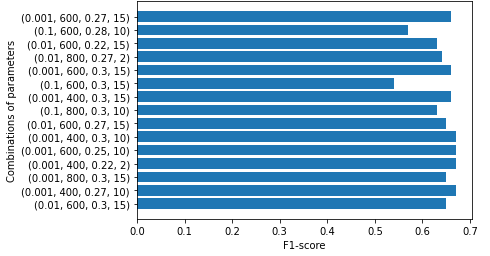
\includegraphics[scale=0.9]{figures/flakycat/parameters.PNG}
\caption{F1 score for different values of parameter combinations using Random Search and a 10-Folds cross-validation. The combinations on the Y axis have the form : (learning rate, number of warm-up steps, similarity margin, support set size). }
\label{fig:parameters}
\end{figure}

\subsubsection{Evaluation metrics}
~~ \\
We use the standard evaluation metrics to compare classifiers, including precision, recall, Matthews correlation coefficient (MCC), F1 score, and Area under the ROC curve (AUC).
These metrics have been used to evaluate the performance of classifiers, including binary classification of flaky tests~\cite{Pinto2020,camara2021use,fatima2021flakify}.
Since our dataset is unbalanced, weighted metrics are more suitable for our evaluation. 

\subsubsection{Research questions}

\begin{itemize}[label={}]
\item \textbf{\textsc{RQ1:}} \emph{How effective is FlakyCat compared to approaches based on other combinations of test representation and classifier?}\\

This question aims to evaluate FlakyCat and compare it to other test representation techniques, \ie vocabulary and test-smell-based and traditional classifiers, \ie SVM, KNN, decision tree and random forest.

\item \textbf{\textsc{RQ2:}} \emph{How effective is FlakyCat in predicting each of the considered flakiness categories?}

This question evaluates FlakyCat's ability to classify the different categories of flakiness.
To perform this, we split the dataset into five sets following the categories: \textit{Async waits}, \textit{Test order dependency},  \textit{Unordered collections}, \textit{Concurrency}, and \textit{Time}.
Then, we use the same settings as for RQ1 to tune the Siamese network, train it, and evaluate it for each category.

\item \textbf{\textsc{RQ3:}} \emph{ How do statements of the test code influence the predictions of FlakyCat?}


We applied the technique we introduced in Section~\ref{sec:flakycat-interpretability} for CodeBERT-based model interpretability to FlakyCat. 
We classified all original short data (323 tests). For 16 tests, the score doesn't decrease by deleting one statement, and thus we collected 307 statements of interest, important for FlakyCat's decision-making. 
To better understand what information emerges, we proceeded with the following analysis. First, we regroup statements by category of flakiness (according to the flaky test they belong to). Then, we want to share information on what type of statements FlakyCat found useful. To do so, we look through the list of statements and attempt to identify recurring code statements and categorize them. The process of identifying statement types is exploratory and inspired by qualitative research. Two of the authors of this paper went through the list of statements and identified nine recurring types of statements:
\begin{itemize}
 \item \textbf{Control flow:} Includes decision-making statements, looping statements, branching statements, Exception handling statements.
 \item \textbf{Asserts:} All types of assertions in tests. 
 \item \textbf{Threads:} statements related to threads and runnables. 
 \item \textbf{Constants:} Constant values such as strings, numbers and boolean values independent of variables, and final variables. 
 \item \textbf{Waits:} All explicit wait statements. 
 \item \textbf{Usage of date/time:} Statements that perform operations on time values, dates. 
 \item \textbf{Network:} Statements related to data exchange in a local or external network between two endpoints, and session management. 
 \item \textbf{I/O:} Statements related to input/output, database and file access. 
 \item \textbf{Global variables:} Includes the use of global variables. 
\end{itemize}

\end{itemize}
With this question, we investigate the prevalence of these statement types in each flakiness category.